% Author: Anwar Baroudi, Rohan Suresh
% Email: mabaroudi@berkeley.edu, rohansuresh@berkeley.edu
% \begin{figure}[H]
% 	\begin{center}
% 		\includegraphics[scale=0.15]{figures/axis.png}
% 	\end{center}
% \end{figure}
\begin{center}
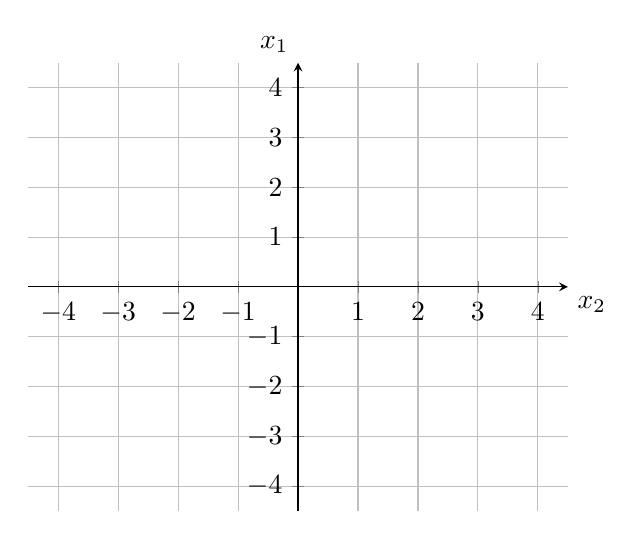
\begin{tikzpicture}[>=latex]
\begin{axis}[
  axis x line=center,
  axis y line=center,
   xtick={-4,...,4},
  ytick={-4,...,4},
  xlabel={$x_2$},
  ylabel={$x_1$},
  xlabel style={below right},
  ylabel style={above left},
  xmin=-4.5,
  xmax=4.5,
  ymin=-4.5,
  ymax=4.5,
  grid]
\end{axis}
\end{tikzpicture}
\end{center}
\[\m{A}=\begin{bmatrix} 1 & 2\\ 1 & 2 \end{bmatrix},\quad \vec{x}=\begin{bmatrix} 3 \\ 1 \end{bmatrix}\]
\begin{enumerate}
\item Draw the space on the figure above that is represented by the span of all the column vectors in $A$. Also draw the space covered by the span of all the row vectors in $A$. What dimension are these spaces?

\answerbox{1cm}

\sol{
The 1 dimensional space for the column space is a line on the $x_2=x_1$ axis (so a diagonal line that goes perfectly northeast, intersecting the origin along the way). The 1 dimensional space for the row space is the line $x_2=2x_1$
}

\note{
Remember that the lines that are drawn are infinite, make sure to make a point of that.
}

\item Consider some arbitrary vector $\vec{v}=\begin{bmatrix}v_1\\v_2\end{bmatrix}$. Write out the product $\m{A}\vec{v}$ in terms of $v_1$, $v_2$, and the columns of $\m{A}$.

\answerbox{1.5cm}

\sol{
\[
    \m{A}\vec{v} = v_1\begin{bmatrix}1\\1\end{bmatrix} + v_2\begin{bmatrix}2\\2\end{bmatrix}
\]
}

\note{
  Make sure students are aware that in general, any matrix-vector product $\mathbf{A}\vec{v}$ can always be written as a linear combination of the columns of $\mathbf{A}$. As such, $\mathbf{A}\vec{v}$ is ALWAYS in the span of the column vectors of $\mathbf{A}$.
}

\item We have talked about how matrices like $\m{A}$ have no inverse. Give a geometric explanation for why this is the case.

\answerbox{1.5cm}

\sol{
If we are given some point on the line for the colspace from part (a), we do not know where it came from. For example, if you gave the point given by $\m{A}\vec{x}$, you have no way of knowing that it came from $\vec{x}$. For example, $\vec{x} = \begin{bmatrix}
1 & 2
\end{bmatrix}^T$ also works.
}

\note{
  Make sure students see the ties between independence/invertibility and the geometry. Geometrically, if we pick a point described by vector $\vec{b}$ on the graph, invertibility would imply that we can always find the unique $\vec{x}$ such that $\mathbf{A}\vec{X} = \vec{b}$.
}

\item Consider all points $\vec{y}$ such that $\m{A}\vec{y} = 0$ Draw the space that the $\vec{y}$'s will make up. What do you notice geometrically? What is the dimension of this space?

\answerbox{2.5cm}

\sol{
This line should be a straight line that is perpendicular to the line for the row space from part (a). It is a space of dimension 1
}

\note{
  This is a good time to note the relationship between the dimension of the column space and the dimension of the null space. You or your students may have heard this referred to as the rank-nullity theorem: for an $m \times n$ matrix $\mathbf{A}$, $$ \text{dim(Col}(\mathbf{A})) + \text{dim(Nul}(\mathbf{A})) = n $$ always holds.
}
\end{enumerate}
